\chapter{Realisieren}\label{ch:realisieren}
In diesem Kapitel wird die IPERKA-Phase Realisieren dokumentiert. Es werden die Wichtigsten und entscheidenen Punkte während der Implentierung festgehalten. 

\section{Backend erweitern}
In diesem Abschnitt wird die Implementierung des Backends dokumentiert. 
\subsection{Neuer REST-Endpunkt}
Als ersten Schritt wurde der neue REST-Endpunkt erstellt:
\begin{lstlisting}[language=Java]
	@JsonApiResource(attributes = Airlock2FAShortActivationCodeData.class)
@Path("activation-code-short")
public Response getShortActivationCode (@ExistingUser @PathParam("userId") @Parameter(schema = @Schema(type = "string")) UserParam userParam) {
	return ok(new Airlock2FAShortActivationCodeData(null)).build();
}
\end{lstlisting}
Der Endpunkt sieht aktuell so aus. Es sind noch keinerlei Funktionalitäten implementiert. Daher wird auch hardcoded null zurückgegeben. Airlock2FAShortActivationCodeData.java ist das Dataobjekt welches ein nullable Feld \flqq short\_activation\_code\frqq{} enthält. \\
\\
\textbf{Rolebased Access Control}\\
Damit der Zugriff auf den neuen Endpunkt nur dann funktioniert, wenn der Admin die nötigen Rollen dazu besitzt, musste eine neue RestAction definiert werden. Diese wird in der Klasse RestActionsDefinitions.java folgendermassen erstellt:
\begin{lstlisting}[language=Java]
	public static RestAction viewAirlock2FAActivationCode () {
	return RestAction
	.builder()
	.action(viewAirlock2FAActivationSecret)
	.rule(Rule.of(GET, "/users/[^/]+/tokens/airlock-2fa/activation-code-short"))
	.build();
}
\end{lstlisting}
Dies bewirkt nun, dass die Action \flqq viewAirlock2FASecrets\frqq{}, welche es schon gab, auf diesen Pfad matched. Das heisst bei jedem Call auf den neuen Endpunkt, wird zuerst validiert, ob der Nutzer die richtigen Rollen hat, welche für diese Action benötigt werden, ansonsten wird 403 zurückgegen.
Ein Problem hat sich nun hervorgehoben. Es gibt bereits folgendes Pattern:\\
 \flqq .rule(Rule.of(GET, "\verb*|text/users/[^/]+/tokens/airlock-2fa(/.*)?"))|\frqq{}
\\
Dieses Pattern matched auch auf den neuen Pfad. Da dieses Pattern in der allgemeine Action \flqq viewToken \frqq{} definiert wurde, könnte es nun zu Konflikten kommen. Deshalb wurde der neue Pfad in diesem Pattern mit Hilfe eines Negative Lookaheads ausgeklammert. Das neue Pattern für die viewToken Action sieht nun so aus:\\


\noindent \verb @/users/[^/]+/tokens/airlock-2fa(?!/activation-code-short(?:/|$))(/.*)?\$ @\\\\
So kann die viewAirlock2FAActivationSecrets Action unabhängig von der viewToken Action konfiguriert werden. Es entstehen dementsprechend keine fehlkonfigurationen und überschreibungen der Mappings.\\
\\
\textbf{REST-Dokumentation}\\
Eine Anforderung an neue REST-Endpunkte ist deren Dokumentation. Zum Zeitpunkt der Probe-IPA wird diese mit Miredot via Javadoc generiert. Sprich Miredot erstellt eine REST-Dokumentation, basiernd auf dem Javadoc. Für den neuen Endpunkt setzt sich diese Dokumentation wie folgt zusammen:
\begin{figure}[H]
	\begin{center}
		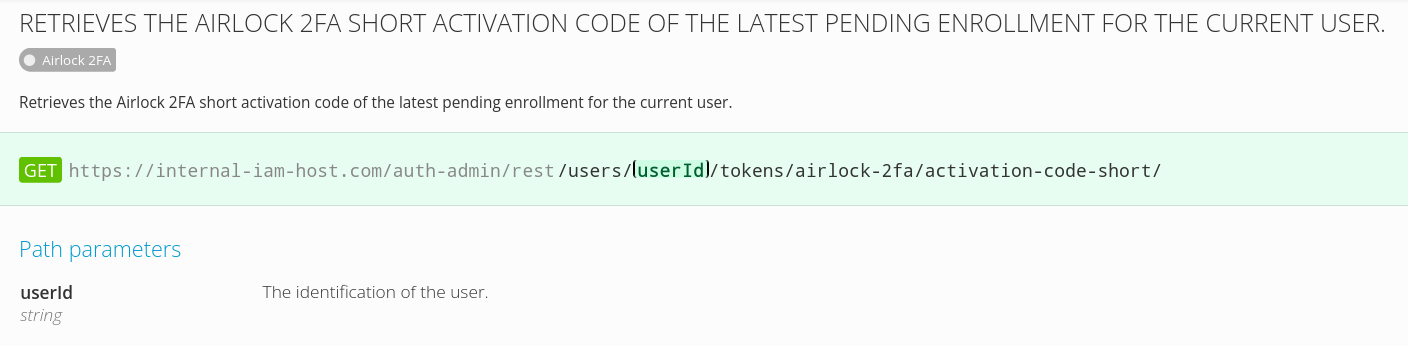
\includegraphics[width=1.0\textwidth]{ressourcen/requestdoc}
		\caption[REST-Dokumentation Request]{Miredot REST-Dokumentation Request}\label{fig:requestdoc}
	\end{center}
\end{figure}
\noindent Zu oberst ist immer der Titel des Requests. Darunter folgt eine Kurze Zusammenfassung. Danach ist der Pfad dargestellt mit der entsprechenden HTTP-Methode.
Zum Schluss folgen die Pfadparamter, was in diesem Fall die User ID ist.
Anschliessend folgt die Response:

\begin{figure}[H]
	\begin{center}
		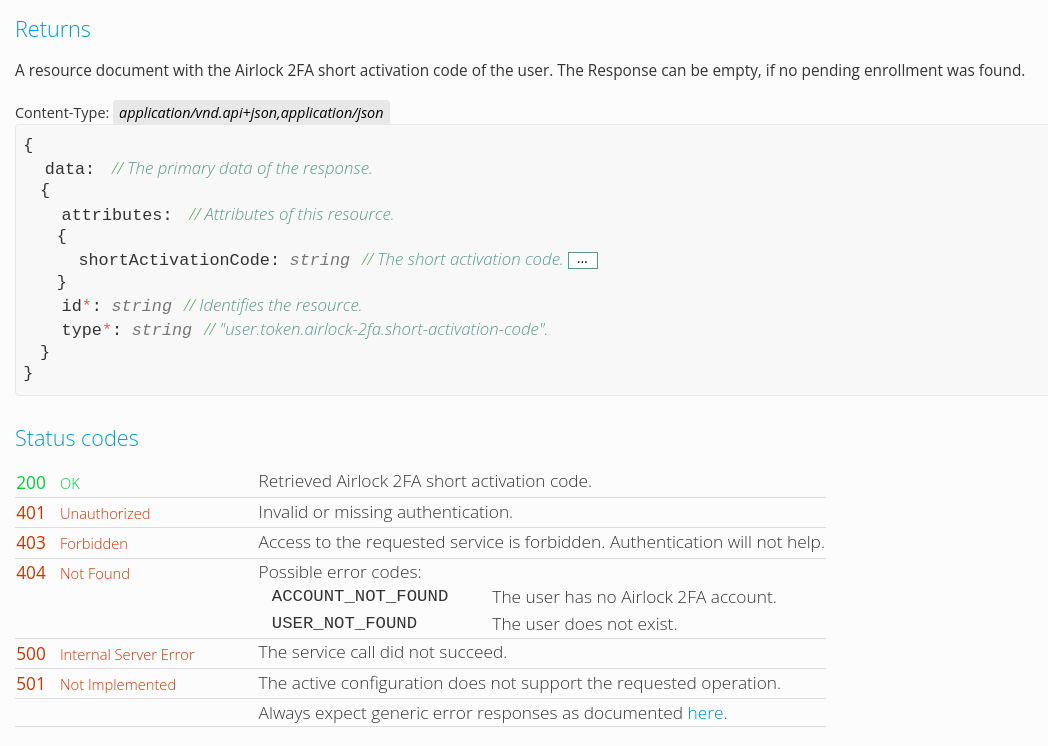
\includegraphics[width=1.0\textwidth]{ressourcen/responsedoc}
		\caption[REST-Dokumentation Response]{Miredot REST-Dokumentation Response}\label{fig:responsedoc}
	\end{center}
\end{figure}

\subsection{Request zu Futurae}



















